\section{Analysis}
\label{sec:Analysis}
\subsection{Data preparation}
Before starting the analysis the given data is being prepared.
Two Monte Carlo data sets are given, one background data set and one containing signal.
Every attribute that is contained in only one of the datasets is being removed as well as Monte Carlo truths, weights and event identification numbers.
In the remaining attributes events that contain the value "inf" or "NaN" are being removed as well.
To differentiate background and signal later labels are being created for the remaining data.
Signal events are being labeled with "1" and background events are being labeled with "0".

\subsection{Feature selection}
The number of the features and the actual features have to be selected before getting into the classifiers.
For that the Jaccard index is calculated depending on the number of features after using the \textit{KNeighborsClassifier}.
This results to a maximum Jaccard index at 20 features.
For the rest of the analysis the best 20 features are determined by the \textit{SelectKBest} method.
The quality of these features is determined with \texttt{f\_classif}.
The data set is being split into test and training subsets to apply the classifier on.

\subsection{Classifiers}
Three different classifiers are used to separate background from signal:
The \texttt{Naive-Bayes} Classifier, the \texttt{RandomForestClassifier} and the \texttt{KNeighborsClassifier} from the \texttt{sklearn} package are being used.

For the \texttt{RandomForestClassifier} a \texttt{RandomForest} with 100 decision trees is being created.
For the classification efficiency, purity and the Jaccard index are being calculated.

For the \texttt{KNeighborsClassifier} the amount of neighbors is set to 20.
It shows that a higher amount of neighbors is not increasing the separating power.

Lastly the \texttt{Naive-Bayes} Classifier is tested on the data set.

All results are shown in table \ref{tab:results}.
The different ROC curves are shown in \ref{fig:roc_curves}.

% RandomForest
% Effizienz: 0.9771 (+/- 0.0057)
% Reinheit: 0.9893 (+/- 0.0033)
% Jaccard Index: 0.9669 (+/- 0.0057)
%
% kNN
% Effizienz: 0.8384 (+/- 0.0080)
% Reinheit: 0.8034 (+/- 0.0068)
% Jaccard Index: 0.6957 (+/- 0.0070)
%
% naive bayes
% Effizienz: 0.7886 (+/- 0.0489)
% Reinheit: 0.8036 (+/- 0.0430)
% Jaccard Index: 0.6605 (+/- 0.0256)

\begin{table}
  \centering
  \begin{tabular}{c | c c c}
    \toprule
    \text{Classifier} & \text{Efficiency} & \text{Purity} & \text{Jaccard index} \\
    \midrule
    \text{RandomForest} & $\num{0.9771(0057)}$ & $\num{0.9893(0033)}$ & $\num{0.9669(0057)}$ \\
    \text{KNeighborsClassifier} & $\num{0.8384(0080)}$ & $\num{0.8034(0068)}$ & $\num{0.6957(0070)}$ \\
    \text{Naive-Bayes} & $\num{0.7886(0489)}$ & $\num{0.8036(0430)}$ & $\num{0.6605(0256)}$ \\
    \bottomrule
  \end{tabular}
  \caption{Efficiency, purity and Jaccard index of the three classifiers applied to the data set.}
  \label{tab:results}
\end{table}


\begin{figure}
  \centering
  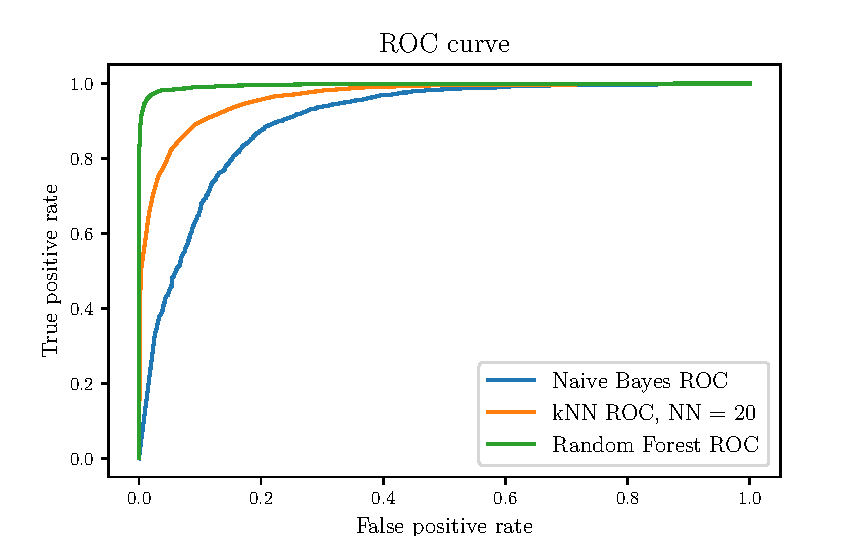
\includegraphics[width=0.8\textwidth]{plots/roc_curve.pdf}
  \caption{ROC-curves of all tested classifiers.}
  \label{fig:roc_curves}
\end{figure}
